\documentclass[
    phd,
    electronic,
    letterpaper,
    simplechapterheading,
    openany,
    parttop,
%    lol,
    lof,
%    lot
]{byumsphd}

\usepackage[
    bookmarks=true,
    bookmarksnumbered=true,
    breaklinks=false,
    raiselinks=true,
    pdfborder={0 0 0},
    colorlinks=false,
    plainpages=false,
]{hyperref}

\usepackage{float}
\usepackage{wrapfig}
\usepackage{enumitem}
\usepackage[all]{hypcap}
\usepackage{amssymb}
\renewcommand{\labelitemi}{\tiny$\blacksquare$}

% These packages allow the bibliography to be sorted alphabetically and allow
% references to more than one paper to be sorted and compressed (i.e. instead
% of [5,2,4,6] you get [2,4-6])
\usepackage[numbers,sort&compress]{natbib}
\usepackage{hypernat}

% Produce nicely formatted paragraphs. There is nothing additional to do.
\usepackage{microtype}

% For UML diagrams
% http://metauml.sourceforge.net/old/index.html
\usepackage{ifpdf,graphicx}
\ifpdf
  \DeclareGraphicsRule{*}{mps}{*}{}
\fi


%%%%%%%%%%%%%%%%%%%%%%%%%%%%%%%%%%%%%%%%%%%%%%%%%%%%%%%%%%%%%%%%%%%%%%%%%%%%%%%

\newcommand{\Title}{Component-based game object system}
\newcommand{\Author}{Nicolas Porter}
\newcommand{\GraduationMonth}{April}
\newcommand{\GraduationYear}{2012}

\committeechair{Dr. Doron Nussbaum}
%\committeemembera{Has~A.~Thought}
%\committeememberb{Wants~A.~Change}
%\committeememberc{Attends~A.~Meeting}
%\committeememberd{Will~B.~Present}

\university{Carleton University}
\universityabbrev{CU}
\department{Computer~Science}
\departmentprefix{School of}
\departmentprefixshort{School}
%\graduatecoordinator{Kent~E.~Seamons}
%\collegedean{Thomas~W.~Sederberg}
%\collegedeantitle{Associate~Dean}

% Set up the internal PDF information so that it becomes part of the document
% metadata.  The pdfinfo command will display this.
\hypersetup{%
    pdftitle=\Title,%
    pdfauthor=\Author,%
    pdfsubject={Directed Studies, Carleton University, School of Computer Science: %
                Document Created \today},%
    pdfkeywords={directed, software, LaTeX},%
}

%%%%%%%%%%%%%%%%%%%%%%%%%%%%%%%%%%%%%%%%%%%%%%%%%%%%%%%%%%%%%%%%%%%%%%%%%%%%%%%

% Rewrite the itemize, description, and enumerate environments to have more
% reasonable spacing:
\newcommand{\ItemSep}{\itemsep 0pt}
\let\oldenum=\enumerate
\renewcommand{\enumerate}{\oldenum \ItemSep}
\let\olditem=\itemize
\renewcommand{\itemize}{\olditem \ItemSep}
\let\olddesc=\description
\renewcommand{\description}{\olddesc \ItemSep}

% Important settings for the byumsphd class.
\title{\Title}
\author{\Author}
\monthgraduated{\GraduationMonth}
\yeargraduated{\GraduationYear}
\yearcopyrighted{\GraduationYear}


% Customize the name of the Table of Contents section.
\renewcommand\contentsname{Table of Contents}

% Remove all widows an orphans.  This is not normally recommended, but in a
% paper dissertation there is no reasonable way around it; you can't exactly
% rewrite already-published content to fix the problem.
\clubpenalty 10000
\widowpenalty 10000

% Allow pages to have extra blank space at the bottom in order to accommodate
% removal of widows and orphans.
\raggedbottom

%%%%%%%%%%%%%%%%%%%%%%%%%%%%%%%%%%%%%%%%%%%%%%%%%%%%%%%%%%%%%%%%%%%%%%%%%%%%%%%

\begin{document}

% Produce the preamble
\microtypesetup{protrusion=false}
\maketitle
\microtypesetup{protrusion=true}



\chapter{Introduction}

% 1. Introduction (1-2 pages)
% 1.1 Motivation
% 1.2 High-level problem description
% 1.3 Overview of results
% 1.4 Paper Organization


\section{High-level problem description}

When someone tries to learn game development, they will usually try to make a relatively small game; one that has a modest game world which contains two or three game objects. The technique that is typically shown in beginner-level game development resources to implement such as game starts by instructing the developer to organize his game objects in a hierarchical manner. The developer then successfully implements the rest of his game. Feeling confident, he tries to add more game object types but quickly discovers that without resorting to ugly coding tricks, he would have to re-engineer his game object hierarchy. Although this works because his game is small,  this technique of organizing game objects in a hierarchy is not compatible with today's game development process because of its inflexibility and maintenance problems which I will describe later in this paper. Furthermore, this system does not allow game object types to be defined in data. This means that the task of adding or removing game object types, as well as modifying a type's behaviors, is left to the software engineers.

A good game object system must be scalable such that game object types can be added easily to the system regardless of the number types already defined. It must also be maintainable such that behaviors can be added to or removed from a game object without problems. Lastly, it should be modular such that game object or their behaviors can be reused for different games.

The hierarchical game object system cannot support those requirements and thus, other approaches need to be explored. The candidate explored in this paper is the component-based game object system which uses composition, rather than inheritance, to define game object types and their behaviors.


\section{Overview of Results}

A hierarchical game object system is easy to understand, but scalability issues arise as the number of game object type increases. The component-based approach presents a solution to these issues, but it is much harder to implement in statically typed languages such as C++.


\chapter{Previous Works}

This chapter lists a few of the more popular component-based game object systems available.


\section{Artemis}

URL: \url{http://www.gamadu.com/artemis/} \\
Language: Java

The architecture of this system is very interesting. The game objects (referred as entities) are simply an id. They are aggregated in an entity manager which maps an entity to its components. The components only encapsulate state; they do not define a behavior. Instead, the behaviors of a game object are defined in what they call systems. A system acts on a subset of an entity's components. For example, the \textit{MovementSystem} would act only on the \textit{velocity} and \textit{position} components of an entity. These systems are stored in what is called a system manager. Individual systems can be retrieved from the system manager. The communication between systems is done via function call.


\section{Cistron}

URL: \url{http://code.google.com/p/cistron/} \\
Language: C++

Cistron is lightweight, fast and flexible. It follows the component-based game object system described in this document fairly closely. Communication is done either by directly calling a method of a component, where the component is retrieved from the game object and the dynamically casted to the appropriate type, or via message passing. As for the state of the game object, it is encapsulated in the components as opposed to being shared as in my implementation.


\section{Craftyjs}

URL: \url{http://craftyjs.com/} \\
Language: Javascript

Because Javascript is a dynamic programming language, it lends itself really well to component-based game object systems. This particular implementation has game objects (referred as entities) which hold their state and components which encapsulate behaviors. Component to component communication is done via event callbacks.


\chapter{Some Definitions}

Before we can talk about various ways to engineer a game object system, we must first define a few terms.


\section{Game Objects}

Game objects represent the actors of the game world. A game object can be either static or dynamic. Static game objects do not react to external stimuli and therefore, do not interact with the world or other game objects. They are often scenery elements, like a tree or a rock. Dynamic game objects, on the other hand, can interact with other game objects.

Arguably, the game camera could be considered a game object because while it does not affect the game world, it is affected by it. For example, a third-person camera needs to react when colliding with geometry in order to avoid clipping.

The Heads' Up Display (HUD) is not a game object since it is not part of the actual game world, it merely displays information about it. Similarly, post-processing effects are not considered game objects because they only affect the rasterized output and not the game world. A game object can have many behaviors, but it must have at least one otherwise it would not be considered a game object since it would be unable to interact with anything in the game world.


\section{Game Object Behaviors}

A behavior describes how a game object reacts to a certain internal or external stimuli. A reaction is the execution of the behavior and may or may not cause side effects in the game world.


\section{Game Object Property}

A game object property is a characteristic of a game object, such as its position or color.


\section{Game World}

The game world contains all game objects. Communication between game objects is performed at this level.


\section{Game Object Model}

The abstract representation of a game that defines the interactions between game objects, the game rules, etc.


\section{Game Object Systems}

The game object system is the part of the game engine that enables the implementation of the game object model. It describes the instantiation of game objects, how to manipulate a game object's state, how to define the behavior of a game object and how game objects communicate with each other. 


\section{Evaluation Criteria}

Here is a list of features that I deem important in any good game object system:


\subsection{Is it easy to add/modify/remove behaviors to/from a game object?}

Drastic changes to the game play model can occur during the development of a game. Therefore, it should be easy to add or remove game object behaviors. The change should also be local to a game object, meaning that it should not require the modification of one or many game object types. Otherwise, it could incur significant maintenance issues. Consequently, the game object system should be designed in a way that does not require dependencies between the behaviors of a game object.

\subsection{Can we reuse game object types, or their behaviors, in new games?}

Game object types and especially behaviors should be as reusable as possible because it will reduce the development time of other games.


\subsection{Is it easy to understand the code/architecture?}

Game development teams are typically large, so many people will have to look at the game objects. Therefore, the code and design must be easy to understand.


\subsection{Does it improve the efficiency of the game development process?}

Can new game object types be built quickly? We also must factor in the development time of the game object system itself. Is it worth the effort?


\subsection{Does the system scale?}

 In other words, how scalable is the system in terms of the number of game objects and the number of behaviors the game object type can define? In order to create rich interactive worlds, modern games typically define many game object types which have many behaviors. A good game object system will allow game developers to define a large number of game objects and behaviors.


\subsection{Can this architecture be defined in terms of data?}

Engineering time is not only expensive, but is also one of the bottlenecks of the game development process. Consequently, game developers create content authoring tools that allow artists, game designers and other non-developers to create content for the game. Not only that, it allows the artist to visualize and tweak his work while the game is running. These content authoring tools can be implemented very easily if most of the game's implementation is defined in data.


\section{Hierarchical / Inheritance-based}

In a hierarchical game object system, game object types are organized in a inheritance hierarchy. More generic game object types lie at the top of the hierarchy, while specialized ones lie at the bottom. The behaviors of a game object type are simply function definitions. This type of model lends itself well to object-oriented programming languages that support inheritance. It was commonly used during the 90's.

It is an easy and intuitive way to model game objects, because it leverages object-oriented concepts that virtually all developers are familiar with. Furthermore, it can be developed relatively quickly from scratch, since most languages used for game development support this system natively. This is why most online tutorials, geared towards beginner game programmers, will feature this architecture.

While it works well for games with simple rules and few game objects, this design does not scale. Firstly, in order to understand a game object type, you must understand its hierarchy. The developer must ensure that by modifying the derived type, he is not violating any assumptions made by parent types. As the number of game object types increases, the hierarchy deepens. It consequently becomes harder to understand a game object type. Furthermore, if a game object type is modified, then its derived types may have to to be modified as well. For example, if we have an \textit{Enemy} interface, and we add the ``runAway()'' behavior to it, then we must implement that behavior in all game object types that implement the \textit{Enemy} interface.

Another scalability problem arises when adding new behaviors to multiple game object types that are in different branches of the hierarchy. This issue is best demonstrated by example. Figure~\ref{fig:hierarchy:1} shows example of a simple game object model implemented using a hierarchical game object system.

\begin{figure}[H]
\bigskip
\centering
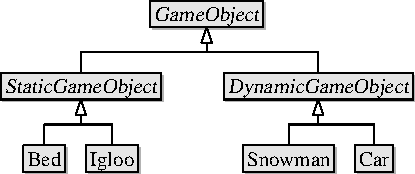
\includegraphics[width=0.8\linewidth]{hierarchy-uml-diagrams/hierarchy-1.pdf}
\caption{A simple game object hierarchy.}
\label{fig:hierarchy:1}
\end{figure}

Let us pretend that during the development of the game, the ``melt'' capability needs to be added to the \textit{Igloo} and \textit{Snowman} types. We could copy the behavior in both types, as shown in Figure~\ref{fig:hierarchy:2}, but that approach is not maintainable because it violates the Don't Repeat Yourself  (DRY) principle.

Alternatively, we could use a mix-in class, as shown in Figure~\ref{fig:hierarchy:3}, but this limits us to a language that supports multiple inheritance, and poses yet another potential maintenance issue. We have already established that in order to understand a game object type, we must understand its hierarchy. But if we use multiple inheritance, the game object type is now part of multiple hierarchies. Therefore, if we want to modify our \textit{Igloo} type, we now have to understand the \textit{StaticGameObject} and \textit{Meltable} hierarchies.

\begin{figure}[H]
\bigskip
\centering
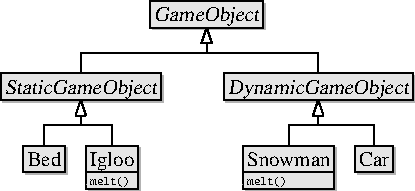
\includegraphics[width=0.8\linewidth]{hierarchy-uml-diagrams/hierarchy-2.pdf}
\caption{Adding the ``melt()" behavior to two types that are in divergent branches.}
\label{fig:hierarchy:2}
\end{figure}

\begin{figure}[H]
\bigskip
\centering
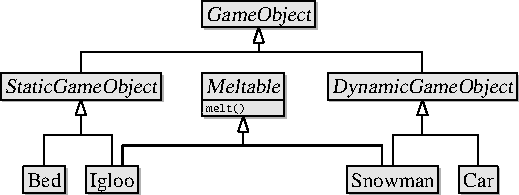
\includegraphics[width=\linewidth]{hierarchy-uml-diagrams/hierarchy-3.pdf}
\caption{Implementing the ``melt()" behavior with a mix-in.}
\label{fig:hierarchy:3}
\end{figure}

What if the game design team suddenly decides that melting makes the game really competitive, and that all game objects should be meltable. How should we implement this new model? We have to move the ``melt()'' behavior upwards in the hierarchy, as shown by Figure~\ref{fig:hierarchy:4}. Alternatively, we could have all types inherit from our \textit{Meltable} mix-in, but that requires us having to modify all existing types. It would not have been a bad approach if we would have implemented our model that way from the very beginning. We will explore this method in Hybrid part of this section.

\begin{figure}[H]
\bigskip
\centering
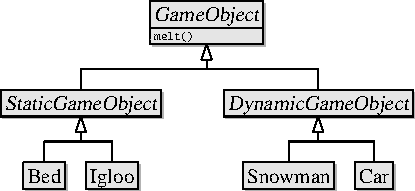
\includegraphics[width=0.8\linewidth]{hierarchy-uml-diagrams/hierarchy-4.pdf}
\caption{Floating the ``melt()" behavior upwards.}
\label{fig:hierarchy:4}
\end{figure}

After testing the new build of the game, the Quality Assurance (QA) team report that the player cannot save his game if he melts his \textit{Bed}, as it is his only save point. But how do we remove the ``melt()'' behavior from our \textit{Bed} type? The \textit{GameObject} type requires us to implement it. We end up removing all logic in the \textit{Bed} such that it is now blank. While that is not a bad solution, it is not ideal as it would be better if the behavior was completely removed.

Finally, this solution is not very modular. Since a game object type defines its own behaviors, it is tightly coupled with many of the engines' subsystems. Take some hypothetical ``draw()'' behavior, for example. It would most likely need to use the graphics subsystem, which means that a game object which implements that behavior will be coupled to the graphics subsystem.

This design does not allow the game objects to be defined in data. All the objects are hardcoded in this hierarchy. This means that software developers must be involved in the addition, modification or removal of game objects. Furthermore, in the case of a compiled language like C++, it means that the system must be recompiled every time a change is made.

If your game requires very few game object types, then this method is not so bad because it implies that the hierarchy is shallow. But for most games, this is not the case.


\subsection{Pros and Cons}

\begin{singlespace}

\begin{minipage}[t]{0.45\textwidth}
\textbf{Pros:}
\begin{itemize}
    \item Simple to understand
    \item Can be developed quickly from scratch
    \item Statically typed
    \item Low overhead
\end{itemize}\end{minipage}
\hfill \vrule \hfill
\begin{minipage}[t]{0.45\textwidth}
\textbf{Cons:}
\begin{itemize}
    \item Not flexible because it is hard to modify game object types after the hierarchy is created.
    \item Hard to maintain as the hierarchy becomes deeper.
    \item Game object may have behaviors they do not need, or should not have.
\end{itemize}\end{minipage}

\end{singlespace}

\pagebreak

\section{Component-Based}

\subsection{Description}

In a component-based system, we flatten the game object hierarchy to a single base game object type which contains a list of behaviors called components. Since the behaviors are decoupled from game objects, the game object system not only becomes much more maintainable, but also very flexible. This system allows us to dynamically compose new game object types, which in turn makes it easy to define them in data. This allows non-developers to create content. One of the first uses of this technique was documented in the \textit{Thief: The Dark Project} postmortem \cite{website:thief}.

\begin{figure}[H]
\bigskip
\centering
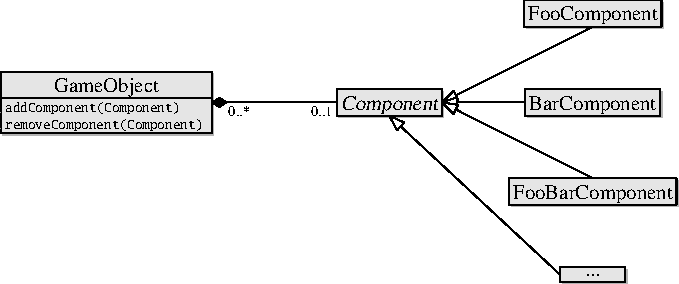
\includegraphics[width=0.8\linewidth]{hierarchy-uml-diagrams/component-3.pdf}
\caption{Game object are composed of many components.}
\label{fig:component:3}
\end{figure}

The key to understand this system is to realize that we are no longer working in the \textit{Object-oriented} paradigm. Game object types are no longer defined in the form of classes. Instead, their type is defined by the set of components they contain. These types are often described in data files and are then instantiated using factory functions. Alternatively, one could create a ``prototype" instance and then clone it when another instance is needed.

Since a game object is composed of multiple parts, as shown in Figure~\ref{fig:components:3}, we have to specify where game object's properties are actually stored. We can either store them in the game object itself, or spread them between the components. Both approaches have their advantages and disadvantages. In any case, it means that whoever holds the properties must expose an interface that will allow components to modify them.

In the case of a game object holding its properties, a property getter and setter must be added to its interface. This means that a component would need a way to retrieve some reference to the game object that owns it, but that is needed regardless due to the component messaging system (seen later). Because we define it dynamically, a game object does not know in advance which properties it will need, which means that there is a risk of property name collisions. For example, if you purchase two components from different manufacturers, and they both use an identical property name but they interpret it differently, your game object may not work properly. One simple solution would be to create a level of indirection between the game object's properties and the affected components.  In a statically-typed language, the data structure backing the properties would need to be implemented as a tagged union. If you are using a dynamically-typed language, a simple associative array (map, dictionary, etc.) would work just fine.

If the properties are to be in held in the game object's components, then a component would need expose its property getters and setters. Then, in order to access or modify a property, a component would have to know which component holds the property. For example, if the \textit{GraphicsComponent} needs the \textit{position} property, it knows that it can get it from the \textit{Movable} component. This approach is not very maintainable because it causes coupling between components. Alternatively, the game object could search each component, but that would be inefficient unless some elaborate caching mechanism is implemented. It is worth noting that while the \textit{Artemis} framework employs this approach, it manages to works around these issues by making components pure data containers.

The game object interface allows components to be dynamically added/removed to/from game objects. This means that a component cannot make any assumptions about other components. Therefore, a component-based game object system must include some messaging subsystem that does not rely on components knowing about each other. A typical way to implement this is via message passing. For example, an \textit{InputComponent} would want to send out a \textit{shoot} message when the player presses the space bar.  While this is a very scalable solution, it does make debugging harder. A common use case of the dynamic component addition and removal feature is that

While this method offers significant advantages over the traditional inheritance-based system, most notably in terms of scalability and maintainability. Unfortunately, it is not easy to develop such a system in a statically-typed language that does not support introspection, such as C++. However, when the system is fully implemented and a library of components is available, adding or maintaining game object types becomes very easy.

\subsection{Pros and Cons}

\begin{minipage}[t]{0.45\textwidth}
\textbf{Pros:}
\begin{itemize}
    \item Scalable, in terms of number of game object types and number of behaviors per game object.
    \item Game object types can be defined in data.
    \item Modular, components can be reused between different games.
    \item After a library of components is assembled, it is easy to make new game object types.
\end{itemize}\end{minipage}
\hfill \vrule \hfill
\begin{minipage}[t]{0.45\textwidth}
\textbf{Cons:}
\begin{itemize}
    \item Building the system takes a lot of time and effort.
    \item Dynamic typing.
    \item While the components themselves are easy to maintain, the component API is not flexible as changing it would require changing all components.
\end{itemize}\end{minipage}


\pagebreak

\section{Hybrid}

\subsection{Description}

We can also create a hybrid from the two types of systems. Instead of using factories to create game object types, behavior interfaces are statically embedded in a generic game object type, and concrete components are injected in the constructor, as shown in Figure~\ref{fig:component:1}. This is could be done by either derived types, or by constructing the game object directly.

\begin{figure}[H]
\bigskip
\centering
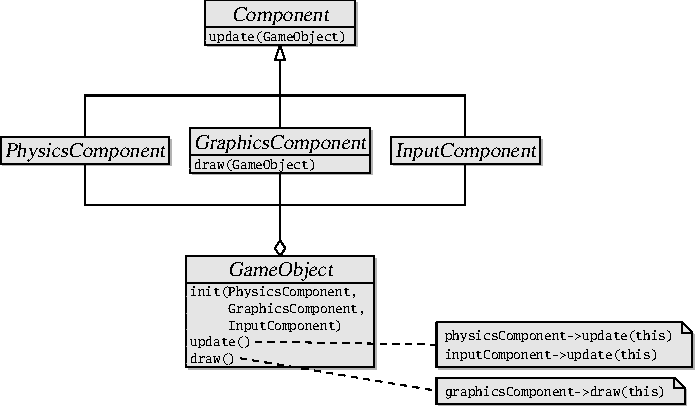
\includegraphics[width=\linewidth]{hierarchy-uml-diagrams/component-1.pdf}
\caption{Hardcoded set of abstract component types in a game object.}
\label{fig:component:1}
\end{figure}

Figure~\ref{fig:component:2} shows how a simple, player-controlled \textit{Snowman} would be implemented. Here, the component implementations would be injected in the game object when it is instantiated. Note that instanciating it this way means that there is no explicit \textit{Snowman} type; the game object is only a \textit{Snowman} by convention. If we wanted to enforce such type, we would need to create one that derives from \textit{GameObject}, and injects the proper components on creation.

\begin{figure}[H]
\bigskip
\centering
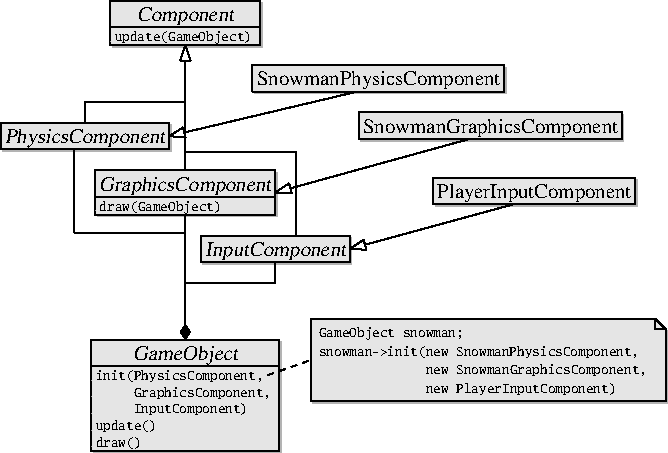
\includegraphics[width=\linewidth]{hierarchy-uml-diagrams/component-2.pdf}
\caption{Snowman game object implemented using components.}
\label{fig:component:2}
\end{figure}

The problems with this approach is that we are loosing a lot of flexibility in terms of game object behaviors, since a class would only support a few select behavior types. That said, those types can be interfaces, which means that it would still allow a game object to change some of its behavior dynamically. It is an attractive solution if you are building a small game, and plan to reuse behaviors between games or you have a library of components already available.

\subsection{Pros and Cons}

\begin{minipage}[t]{0.45\textwidth}
\textbf{Pros:}
\begin{itemize}
    \item Statically typed.
    \item Ability to change certain types of behaviors.
    \item Flexibility of components without the complexity of the system's implementation.
\end{itemize}\end{minipage}
\hfill \vrule \hfill
\begin{minipage}[t]{0.45\textwidth}
\textbf{Cons:}
\begin{itemize}
    \item Similar to the ones outlined in the hierarchical system.
\end{itemize}\end{minipage}


\chapter{Implementation}

\section{Instructions}

Installation instructions can be found in the \textit{README} file that was distributed with the implementation package.

\section{Description}

This paper also presents an implementation of a game object system. This implementation is written in C++, and is heavily reliant on the QT SDK (Software Development Kit). QT enables introspection of C++ objects through its dynamic property system. It does so by using a compiler, MOC (Meta-Object Compiler) which generates vanilla C++ code from C++ code that is annotated with special macros (the Q\_OBJECT macro). It essentially turns C++ into a static/dynamic hybrid language.

In the component system implementation, game objects hold a list of components and a property map which is provided by QT. When a component is added to a game object, it injects the properties that it needs in the game object. However, care must be taken to avoid property name collisions, as there are no coping mechanisms. A rule of thumb is to inject a property only if you would normally have a data member for it in a game object hierarchy. For example, a \textit{Movement} component would most likely have a \textit{position} data member, so it should inject the \textit{position} property. A \textit{GraphicsComponent} may need to access the \textit{position} property, but it shouldn't inject it in the game object.

\begin{figure}[H]
\bigskip
\centering
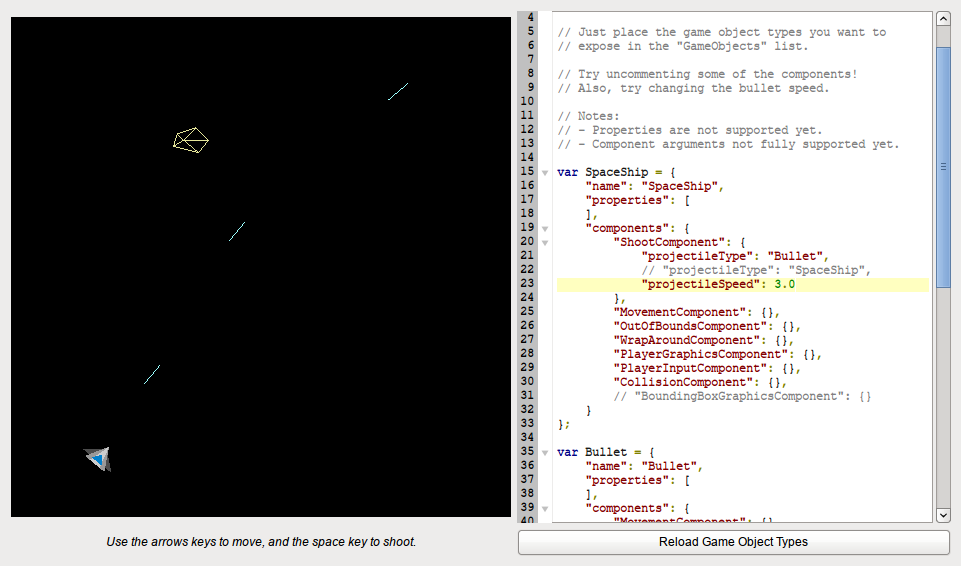
\includegraphics[width=\linewidth]{images/implementation-screenshot.png}
\caption{A screen shot of a game that uses the component-based game object system implementation, as well as the component editor. }
\label{fig:implementation:1}
\end{figure}

As Figure~\ref{fig:implementation:1} shows, a sample game has been built with the component system. The implementation also features a component data file editor which enables you to dynamically modify game object types. The format of the game object type configuration file is in Javascript. This could allow interesting type generation, however that is not demonstrated in the sample configuration file provided with the implementation.

Interpreting this configuration file yields intermediary data structures called \textit{descriptors}. There are two types of descriptors: a \textit{ComponentDescriptor} and a \textit{GameObjectDescriptor}. The purpose of these structures is to decouple the encoding of the configuration file from the game engine's configuration interpreter. These descriptors are stored in\textit{string} to \textit{descriptor} maps that reside in \textit{instanciators}. The purpose of the instanciators is to expose an API that allows the instanciation of an object from a string. In other words, they are factories. There are two types of \textit{instanciators}: a \textit{GameObjectInstantiator} and a \textit{ComponentInstanciator}. The \textit{GameObjectInstanciator} first creates a new game object, and then matches the \textit{string} to a \textit{GameObjectDescriptor}, which contains a list of \textit{ComponentDescriptor} instances. A \textit{ComponentInstanciator} is then used to these descriptors, and the resulting component instances are added to the game object.

The game object API allows components to be added or removed dynamically. Components hold an \textit{owner} reference which points to the game object that contains it. Derived components will rarely use the reference directly since most of the game object API calls are wrapped by the abstract \textit{Component} class, to reduce coupling and to increase maintainability.

Amongst other things, components are able to mark their owner for deletion. This is useful when you want to delete an object after a certain event occurs, for example when an object runs out of health and should disappear as a result. In the sample game provided with the implementation, this functionality is used when a collision occurs between an \textit{Asteroid} and a \textit{Bullet}.

The component communication system is implemented using message passing, where the game object is used as a message bus for component communication. A component registers certain messages upon insertion in a game object. This is just an optimization to prevent relaying messages to components that would not need to capture them. An example of message passing can be found in the \textit{ShootComponent} and \textit{PlayerInputComponent}. Basically, when the player presses the \textit{space} key, the \textit{PlayerInputComponent} fires a \textit{shoot} event, which is the captured by the \textit{ShootComponent}.


\chapter{Conclusion}

\section{What was achieved}

This paper analyzed and described the differences between hierarchical and component-based game object systems, and pointed out the pros and cons of those schemes.

It was concluded that component-based game engine systems are more maintainable and scalable than hierarchical ones. Furthermore, it allows the definition of game object types in terms of data, which is a desirable property of a game object system because it enables the development of content authoring tools.

It also presented an implementation of a component-based game object system, as well as a sample asteroids-like game that is built with it. The interface also features a simple game object type editor, to illustrate that game object types can indeed be defined in data and modified dynamically.


\section{Future work}

More work needs to be done to find a clean way to integrate components in other game engine subsystems. I believe that the approach employed by the \textit{Artemis} framework is very close to an optimal solution. The behaviors (called \textit{systems}) can be completely stateless, which means that more complex behaviors can be built by just composing systems.

The QT SDK's scripting capabilities, where Javascript code can be used to call native C++ code, should be explored. This feature is supposed to change drastically in QT's next version (5.0), which is why I did not use it for my implementation. It would allow me to implement components directly in data.

Another area that would be worth exploring is node-based visual programming user interfaces used for the development of game object types, component to component communication and even gameplay rules. Figure~\ref{fig:node-editor} shows an interface prototype that I was working for this project, but did not have a chance to complete.

\begin{figure}[H]
\bigskip
\centering
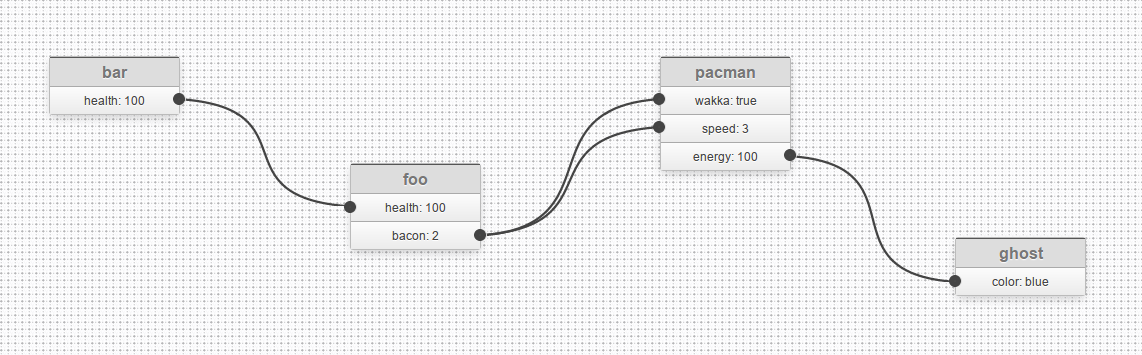
\includegraphics[width=\linewidth]{images/node-editor.png}
\caption{Prototype of a node-based visual programming interface for game object type creation.}
\label{fig:node-editor}
\end{figure}

% 5.1 what addressed in paper
% 5.2 What was achieved
% 5.3 Benefits
% 5.4 Future work

\nocite{*} 


\bibliographystyle{plainnat}
\bibliography{bib}

\end{document}

